\documentclass{beamer}
\usetheme{Berkeley}
\usecolortheme{dove}
\title{A review of Kirchner in Shyft hydrology}
\subtitle{Based on: Catchments as simple dynamic systems: Catchment characterization, rainfall-runoff modeling, and doing hydrology backward by James W. Kirchner, published in Water Resources Research, vol. 45, W02429, doi: 10.1029/2008WR006912, 2009}
\author[]{c++ impl. by Phd Ola Skavhaug, \\
	reviewed by MSc Sigbjørn Helset}
\begin{document}
\begin{frame}[plain]
    \maketitle
\end{frame}
\section{introduction}
\begin{frame}{Introduction}
	\emph{This presentation was initiated after questions from the operational use of Shyft hydrology, where users experienced very low responses from the Kirchner-routine, even in large rainfall events. \\
	As per usual, we use that as an opportunity to verify and check all of our assumptions regarding implementation and use.\\
	 The reviewer found the original Kirchner article well written, worth re-reading, -several times.\\
	 The c++ implementation is also very robust, efficient, commented and well suited for the purpose. The test-coverage is good, and also contained the needed checks/experiments that led up to our current implementation.}
\end{frame}
\subsection{content}
\begin{frame}{Content}
	\emph{In this presentation, we take a short trip through the essential parts of the Kirchner paper that directly or indirectly transforms into the implemented c++ code.\\
		 This means that it is not a replacement or summary of what the Kirchner paper covers.\\
		 We strongly encourage hydrologist and researchers to read the paper thoroughly, as it both covers the background, limitations and possible extensions/fixes for those. We hope however, that it is a contribution to ease understanding the c++ implementation, and serve as basis for future developments. }
\end{frame}
\section{theory}
\subsection{mass balance}
\begin{frame}{1. Catchment mass balance}
		\begin{equation}
		\dfrac{ds}{dt} = p -e -q 
		\end{equation}
	
	\emph{The catchment stored water rate-of-change is equal to the incoming precipitation minus evapotranspiration and discharge}\\
	
\end{frame}
\subsection{observation}
\begin{frame}{2. Catchment discharge}
	\label{F:1}
	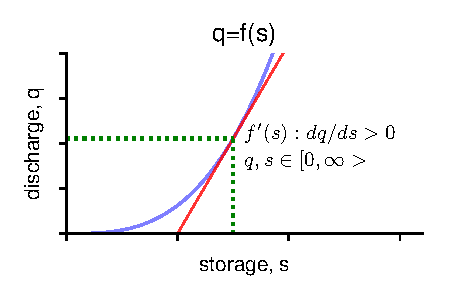
\includegraphics{kirchner_fig1.pdf}
	\\
	
	\emph{\textbf{Keypoint}:The discharge q is a unique function of catchment storage s}
\end{frame}
\subsection{diff eq}
\begin{frame}{3. Working with the equations}
	%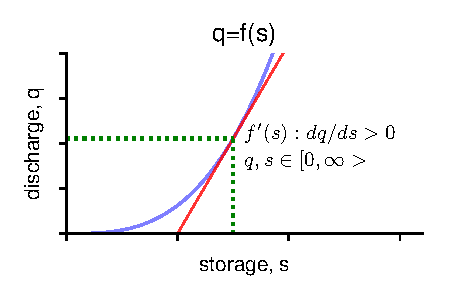
\includegraphics{kirchner_fig1.pdf}
	\begin{equation}
	s= f^{inv}(q)
	\end{equation}
	\begin{equation}
	 \dfrac{dq}{ds}= f'(s) = f'(f^{inv}(q)) = g(q)
	\end{equation}
	\begin{equation}
	\label{eqn:diff_eq}
	\dfrac{dq}{dt}= \dfrac{dq}{ds}  \cdot  \dfrac{ds}{dt} = \dfrac{dq}{ds}(p-e-q) = g(q) \cdot (p-e-q)
	\end{equation}
	\emph{\textbf{Keypoint}:A differential equation, expressed in \textbf{observable} q, q',p,e (not s).}\\
	
	-Now we only need to find a suitable g(q) from the observations.

\end{frame}
\subsection{squeeze observations}
\begin{frame}{We can observe q..}
	Recall equation \ref{eqn:diff_eq} on previous slide:
	\begin{equation}
		\dfrac{dq}{dt}=g(q) \cdot (p-e-q)
	\end{equation}
	And let's see what happens in periods where p-e is very small compared to q
	\begin{equation}
	\Downarrow  p-e \textless\textless q
	\end{equation}
	\begin{equation}
		\dfrac{dq}{dt}=-g(q) \cdot q
	\end{equation}
	\begin{equation}
	g(q)= -\dfrac{\dfrac{dq}{dt}}{q}
	\end{equation}
\end{frame}
\subsection{Empirical g(q)}
\begin{frame}{"The empirical shape of g(q)"}
	\begin{columns}
		\begin{column}{.45\textwidth}
	        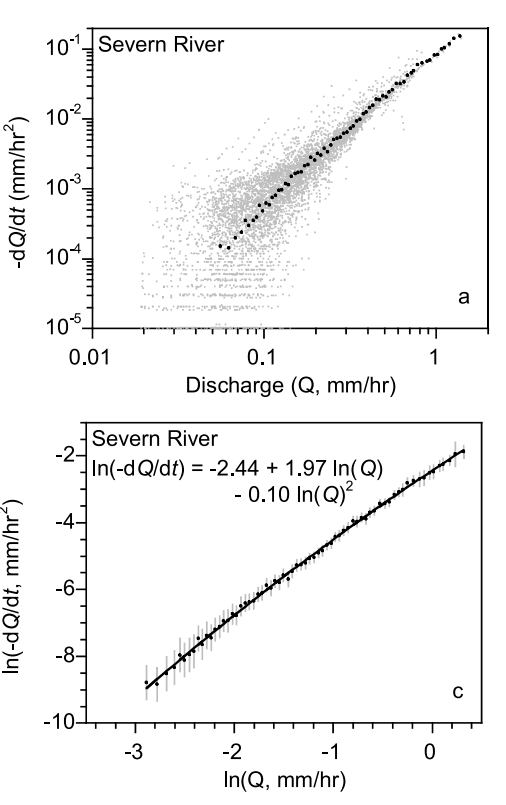
\includegraphics[width=5cm,height=8cm,keepaspectratio]{kirchner_severn_river_fig2.png}
	    \end{column}
        \begin{column}{.45\textwidth}
			Kirchner used observed q and ~q', for period where (p-e) \textless\textless q, and plotting log(dq/dt) vs. log(q) and found/selected:
			\begin{equation}
			g(q)=e^{c_1+ c_2 \cdot ln(q)+ c_3 \cdot ln^{2}(q)}
			\end{equation}
			\emph{It is simple enough and have correct unique g(q) properties when q \textgreater 0}
		\end{column}
	\end{columns}
\end{frame}
\section{implementation}
\subsection{log transform}
\begin{frame}{Formulating diff. eqn. for numerical solver I}
	\begin{equation}
	\dfrac{d ln(q)}{dt}=\dfrac{1}{q} \cdot \dfrac{dq}{dt}=g(q) \cdot (\dfrac{p-e}{q}-1)
	\end{equation}
	\begin{equation}
	\Updownarrow  \dfrac{1}{q}= e^{-ln(q)}, q \textgreater 0 \nonumber
	\end{equation}
	\begin{equation}
	\dfrac{d ln(q)}{dt}= g(q) \cdot ((p-e) \cdot e^{-ln(q)}-1)
	\end{equation}
\end{frame}
\subsection{the ODE formula}
\begin{frame}{Formulating diff. eqn. for numerical solver II}
	\begin{equation}
	\dfrac{d ln(q)}{dt}= e^{c_1 + c_2 \cdot ln(q)+ c_3 \cdot ln^{2}(q)} \cdot ((p-e) \cdot e^{-ln(q)}-1)
	\end{equation}
	\begin{equation}
	\Updownarrow  q_{x}=ln(q) \nonumber
	\end{equation}
	\begin{equation}
		\dfrac{d q_{x}}{dt}= e^{c_1+ c_2 \cdot q_{x}+ c_3 \cdot q_{x}^{2}} \cdot ((p-e) \cdot e^{-q_{x}}-1)
	\end{equation}
	\emph{This equation is expressed on kirchner.h:201:log\_transform\_f()}
\end{frame}
\subsection{c++}
\begin{frame}{cpp/shyft/hydrology/methods/kirchner.h}
	\begin{enumerate}
		\item Using boost::nummeric::ode package to solve ln(q)-transformed ODE \url{https://www.boost.org/doc/libs/1_71_0/libs/numeric/odeint/doc/html/index.html}
		\item Using runge-kutta-dopri5 stepper
		\item Integrate using trapezoidal-average found to be accurate enough
	\end{enumerate}
To avoid singularity area very close to q=zero: 
	\begin{enumerate}
		\item If q is less than 0.00001mm, we return 0.0
		\item If $g(ln(q)) < 1E-30$, then $ \dfrac{dx}{dt}=0 $
	\end{enumerate}
\end{frame}
\section{Experience and feedback}
\begin{frame}
	\textbf{Overall experience}: It just works!\\
	\textbf{Adjustments}: In operation we experienced q==0, so we introduced the limits as specified, to avoid singularities and maintain reasonable results.\\
	\textbf{Missing response on low q}: This is by design, determined by the parameters(c1..c3). Have a look at kirchner figure 13. Illustrating very different responses for same 20mm/hr rain event. Idea: maybe we should set lower limit q to the lowest response/sensitivity wanted for the catchment?\\
\end{frame}
\section{Next steps}
\begin{frame}{Next steps and improvements}
	\textbf{Calibration vs. estimation} Kirchner uses estimation based on observation to determine c1..3. Shyft allow for calibration, easy and often used using a starting point for c1..3. Should we combine that with estimation approach to ensure robust behavior for q outside calibrated range ?\\
	
	\textbf{Understanding c1..c3} Is really about understanding the g(q), and and the selected response function, driven from the observations of q.\\
	
	\textbf{What about snow and cells, not catchments?}: Does it work, is it entirely positive. Dry during winter, and suitable in spring/melt season? Does height distribution work well, melt and kirchner response in low land, dry up in cold mountains? \\
	
	\textbf{Algorithm development}: Kirchner points out several possible extensions, should we explore some of those ?
	
\end{frame}
\end{document}
